\section{Routing Characterization}
\label{sec:iib}

The clairvoyant-comparator-gap analysis measured a substantial miss-byte gap between Global-LRU
and the implemented clairvoyant Belady-style comparator $O_B$ under
constrained memory (Sections~\ref{sec:oracle-headroom}--\ref{sec:recoverable-envelope}).
After \textsc{AUDIT-ORACLE-001}, that comparator gap is not interpreted as a
proven byte-optimal bound or a proven upper bound on causal recovery; it
shows separation from a non-causal comparator, not whether a causal policy
can close it. This section asks the necessary prior question:

\begin{quote}
\emph{Is MoE expert routing sufficiently structured, local, and
workload-dependent to justify attempting causal working-set prediction?}
\end{quote}

This is a descriptive characterization stage. It does \emph{not}
answer whether a predictor works, whether prefetch improves runtime,
whether a new retention policy reduces the measured clairvoyant-comparator
gap or improves on selected causal baselines, whether inference
becomes faster, or whether the result generalizes across models. Those
questions belong to the causal-prediction and real-runtime validation
stage or later work.

\subsection{Evidence Base and Scope}
\label{sec:iib-scope}

Table~\ref{tab:iib-map} lists the four canonical PASS experiments.
R-05--R-07 are offline analyses over the same validated R-01 coding
trace used throughout the clairvoyant-comparator-gap analysis
(the canonical trace identified by H-TRACE-R01; Appendix~\ref{sec:hash-registry}),
with layer-local expert identity, no new model/runtime invocation, and no
new trace capture. R-08 adds controlled captures for four workload
families (coding, reasoning, summarization, instruction), two replicates
each, under a fixed Qwen3-30B-A3B-Q4\_K\_M / 4~GiB expert-budget
consumer-machine protocol with deterministic decoding
(temperature~$=0.0$, top-$k=1$). One \code{coding-v1/seed-42} cell reuses the
canonical R-01 trace; seven cells were newly captured for R-08. All
analysis is layer-local and descriptive.

\begin{table}[t]
\centering
\caption{Routing-characterization experiment map (canonical PASS evidence only).}
\label{tab:iib-map}
\small
\begin{tabularx}{\linewidth}{@{}l >{\raggedright\arraybackslash}p{2.9cm}
  >{\raggedright\arraybackslash}X l l@{}}
\toprule
Exp. & Question & Primary metrics & Run & Outcome \\
\midrule
R-05 & Expert frequency and concentration & normalized entropy, effective experts, top-8 share, 80\% mass & \texttt{da82e15b61c9\ldots} & PASS \\
R-06 & Routing transition structure & same-layer NMI, conditional entropy, self-transition lift & \texttt{2e075161f024\ldots} & PASS \\
R-07 & Reuse distance and working-set structure & reuse fractions, gaps, distinct-intervening distance, working set, shuffled null & \texttt{af28e8c6dc50\ldots} & PASS \\
R-08 & Routing drift and workload dependence & temporal/replicate/cross-workload JSD, top-8 Jaccard distance, regime & \texttt{6165471a1257\ldots} & PASS \\
\bottomrule
\end{tabularx}
\end{table}


\paragraph{R-08 capture-provenance audit.}
In the canonical R-08 capture matrix, the reused
\code{coding-v1/seed-42} cell records the run identifier and capture
source of the upstream R-01 capture, while the seven
R-08-managed new captures carry a null run identifier and a null capture
source. This is treated as an intentional
provenance representation of R-08-internal captures, not as a missing
scientific trace: every canonical cell records a trace path, trace
digest, workload identity, seed, model digest, runtime digest,
configuration fingerprint, validation state, and canonical status, all
bound to the canonical R-08 run and its canonical digest
(H-R08-CANONICAL; Appendix~\ref{sec:hash-registry}).
The paper freeze does not invent capture IDs and does not modify
scientific traces.

\subsection{R-05: Expert Frequency and Concentration}
\label{sec:r2-05}

R-05 measures aggregate layer-local routing frequency on the validated
trace. Table~\ref{tab:r2-05-summary} and Figure~\ref{fig:b1-concentration}
summarize the result.

\begin{table}[t]
\centering
\caption{R2-05 expert frequency and concentration summary (descriptive, layer-local).}
\label{tab:r2-05-summary}
\small
\begin{tabular}{@{}lr@{}}
\toprule
Quantity & Value \\
\midrule
Total routing requests (token-expert assignments) & 205,048 \\
Layers / nominal experts per layer / top-$k$ & 48 / 128 / 8 \\
Median normalized entropy & 0.8522 \\
Median effective expert fraction & 0.5136 \\
Median effective experts ($\approx$) & 65.7 / 128 \\
Median top-8 traffic share & 0.3001 \\
Top-8 share range (min--max) & 0.1595--0.4074 \\
Median experts for 80\% traffic & 43 \\
80\% mass range (min--max experts) & 31--68 \\
Most / least concentrated layer & 31 / 0 \\
\bottomrule
\end{tabular}
\end{table}


\begin{figure}[t]
\centering
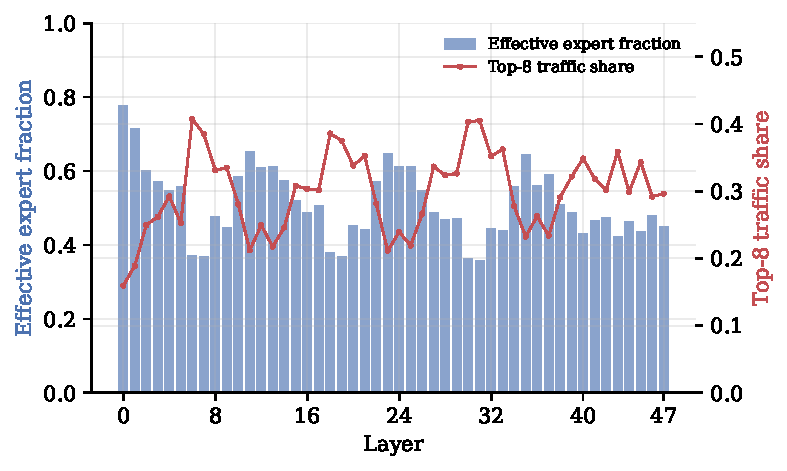
\includegraphics[width=0.78\linewidth]{figures/figure_b1_r2_05_concentration.pdf}
\caption{Layer-wise R-05 routing concentration on the validated coding
trace. Bars show effective expert fraction (effective experts divided by
128 nominal experts); the line shows top-8 traffic share per layer. The
figure measures aggregate non-uniformity across layers, not temporal
stability and not cache performance.}
\label{fig:b1-concentration}
\end{figure}

Across 205,048 token-expert assignment observations, routing is strongly
non-uniform at the aggregate level: the median effective expert fraction
is $0.514$ (about $65.7$ of $128$ nominal experts), the median top-8
traffic share is $0.300$, and the median number of experts required for
80\% of traffic is $43$ (range $31$--$68$).

This concentration does not imply that static frequency-based LFU is a
sufficient retention policy in the tested pressure regime. R-03's
canonical auxiliary evidence shows that static LFU incurs more miss bytes
than Global-LRU at every tested capacity-constrained budget from 1.5 to
8~GiB on the same DEV trace, tying at 16~GiB
(Table~\ref{tab:r2-03-lfu-aux}). Thus substantial aggregate frequency
concentration exists, but static frequency-based LFU does not outperform
recency-based Global-LRU anywhere in the tested pressure regime on this
trace and budget grid. This motivates examining temporal and sequential
information beyond aggregate frequency. R-06 and R-07 test complementary
sequential and temporal structure.

\subsection{R-06: Routing Transition Structure}
\label{sec:r2-06}

R-06 asks whether the previous same-layer routing state carries
information about the next same-layer routing state beyond marginal
frequency. The unit is a \emph{pairwise set-to-set transition
observation}: for consecutive token selections in a layer, every expert in
the source top-8 selection is paired with every expert in the target
top-8 selection. The resulting 1,637,312 observations are therefore
pairwise transition observations generated by top-8 $\times$ top-8
relationships; they are \emph{not} 1.64~million independent samples.

\begin{table}[t]
\centering
\caption{R2-06 routing transition structure summary (same-layer, pairwise set-to-set observations).}
\label{tab:r2-06-summary}
\small
\begin{tabular}{@{}lr@{}}
\toprule
Quantity & Value \\
\midrule
Pairwise set-to-set transition observations & 1,637,312 \\
Layers / nominal experts per layer & 48 / 128 \\
Median same-layer NMI & 0.0989 \\
NMI range (min--max) & 0.0826--0.1368 \\
Layers with positive NMI & 1.00 \\
Median conditional entropy & 3.7353 \\
Median self-transition lift & 4.1850 \\
Median top-1 outgoing probability & 0.0904 \\
Median outgoing effective-target fraction & 0.7170 \\
Maximum supported transition lift (layer) & 31.90 (L37) \\
Strongest / weakest NMI layer & 37 / 45 \\
\bottomrule
\end{tabular}
\end{table}


\begin{figure}[t]
\centering
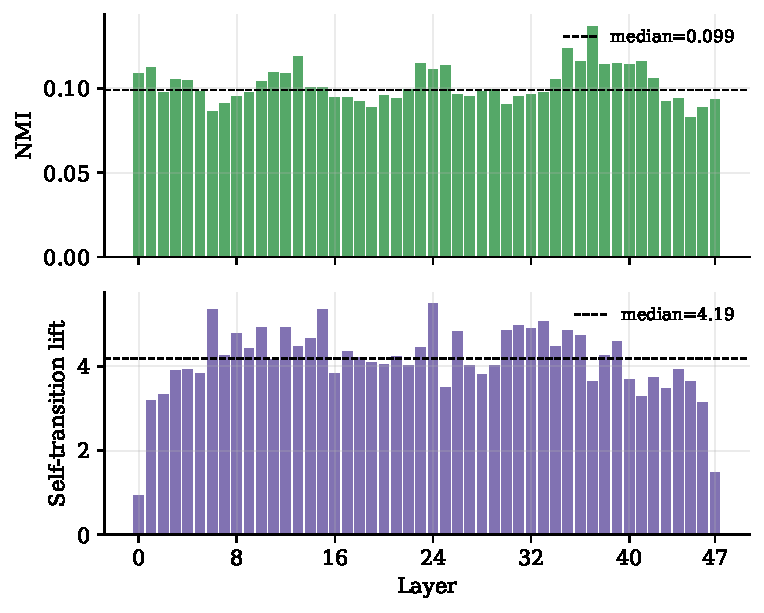
\includegraphics[width=0.78\linewidth]{figures/figure_b2_r2_06_transitions.pdf}
\caption{R-06 same-layer transition structure by layer. Top: normalized
mutual information (NMI) between consecutive token-to-token expert
selections. Bottom: median self-transition lift. Dashed lines mark medians
across layers. NMI measures measurable dependence, not predictor accuracy.}
\label{fig:b2-transitions}
\end{figure}

Table~\ref{tab:r2-06-summary} and Figure~\ref{fig:b2-transitions} show
measurable sequential dependence in every tested layer (fraction with
positive NMI $=1.0$). Median NMI is $0.099$ (range $0.083$--$0.137$),
with median conditional entropy $3.735$. This means the previous routing
state provides a measurable reduction in uncertainty about the next
routing state at the measured resolution. NMI is not translated into
prediction accuracy, and R-06 does not train or evaluate a predictor.

\subsection{R-07: Reuse Distance and Working-Set Structure}
\label{sec:r2-07}

R-07 measures layer-local reuse distance and working-set growth, and
compares observed routing to a deterministic shuffled null that preserves
marginals while destroying temporal order. Table~\ref{tab:r2-07-summary}
and Figure~\ref{fig:b3-reuse} summarize the result.

\begin{table}[t]
\centering
\caption{R-07 reuse distance and working-set summary (observed vs deterministic shuffled null).}
\label{tab:r2-07-summary}
\small
\begin{tabular}{@{}lr@{}}
\toprule
Quantity & Value \\
\midrule
Reuse events / first observations & 199,784 / 5,264 \\
Median immediate reuse (gap=1) & 0.4256 \\
Median reuse $\le 4$ / $\le 16$ positions & 0.6415 / 0.8602 \\
Median token reuse gap / p90 gap & 2 / 24 \\
Median distinct-intervening reuse distance & 8 \\
Median working set $W_8/W_{32}/W_{128}/W_{256}$ & 30.0/57.0/89.5/102.5 \\
Frequency--reuse-gap Spearman (descriptive) & -0.6506 \\
Immediate reuse: observed / null / ratio & 0.4256 / 0.1873 / 2.27$\times$ \\
Reuse $\le 4$: observed / null / ratio & 0.6415 / 0.4780 / 1.34$\times$ \\
Reuse $\le 16$: observed / null / ratio & 0.8602 / 0.8208 / 1.05$\times$ \\
Median gap: observed / null & 2 / 5 \\
Distinct-intervening: observed / null & 8 / 24 \\
\bottomrule
\end{tabular}
\end{table}


\begin{figure}[t]
\centering
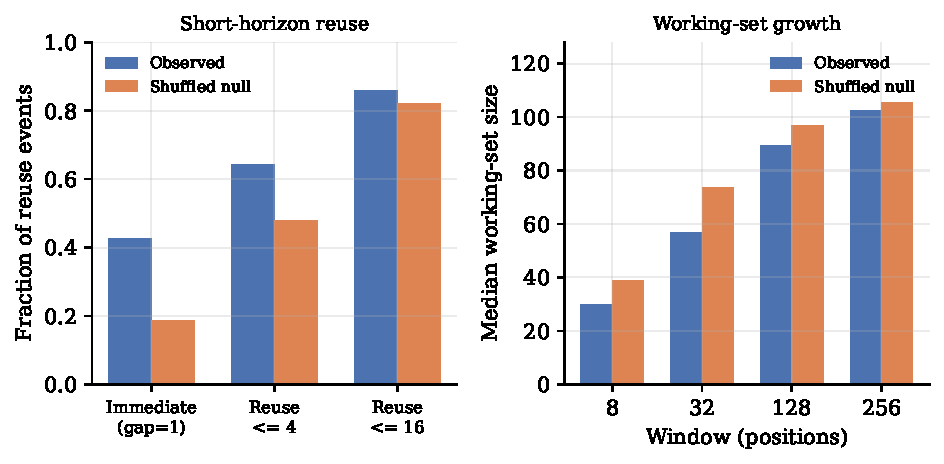
\includegraphics[width=0.92\linewidth]{figures/figure_b3_r2_07_reuse_locality.pdf}
\caption{R-07 observed routing locality versus a deterministic shuffled
null. Left: fraction of reuse events at immediate, $\leq 4$, and
$\leq 16$ position horizons. Right: median working-set size at windows
$W_8, W_{32}, W_{128}, W_{256}$. The departure from the null is strongest
at short horizons, consistent with temporally local structure.}
\label{fig:b3-reuse}
\end{figure}

Observed reuse is concentrated at short horizons. Immediate reuse is
$0.426$ versus $0.187$ for the shuffled null ($2.27\times$); reuse within
4 positions is $0.642$ versus $0.478$; reuse within 16 positions is
$0.860$ versus $0.821$. The observed median token reuse gap is $2$
(null $5$), and the observed median distinct-intervening reuse distance is
$8$ (null $24$). Working sets are smaller than the null at short and
medium windows ($W_8$: $30$ vs.\ $39$; $W_{32}$: $57$ vs.\ $73.5$;
$W_{128}$: $89.5$ vs.\ $97$; $W_{256}$: $102.5$ vs.\ $105.5$).

The strongest departure from the null occurs at short horizons and
narrows at longer horizons. This is a descriptive locality result, not a
prediction result. It motivates short-horizon causal prediction as the
scientifically relevant next test.

\subsection{R-08: Routing Drift and Workload Dependence}
\label{sec:r2-08}

R-08 tests whether routing structure is stable within a workload over
time, reproducible under the same workload and protocol, and dependent on
workload category. The canonical matrix has four workloads
(\texttt{coding-v1}, \texttt{reasoning-v1}, \texttt{summarization-v1},
\texttt{instruction-v1}) with two replicates each, all valid, using the
same model SHA, runtime SHA, and compatible configuration fingerprints.
Comparisons use a matched decode horizon $H=388$ and 8 temporal windows of
length 48.

\begin{table}[t]
\centering
\caption{R2-08 routing drift and workload-dependence scale comparison.}
\label{tab:r2-08-summary}
\small
\begin{tabular}{@{}lr@{}}
\toprule
Quantity & Value \\
\midrule
Matrix & 4 workloads $\times$ 2 replicates = 8 cells \\
Reused / new captures & 1 / 7 \\
Matched decode horizon $H$ & 388 \\
Temporal windows / window length & 8 / 48 \\
Median temporal JSD & 0.135556 \\
Median same-workload replicate JSD & 0.0\,\footnotemark[1] \\
Median cross-workload JSD & 0.299496 \\
Cross-workload / temporal ratio & 2.2094$\times$ \\
Median top-8 temporal Jaccard distance & 0.606061 \\
Predeclared regime & WORKLOAD\_DEPENDENCE\_DOMINANT \\
Most / least stable workload & instruction-v1 / coding-v1 \\
Most / least stable layer & 47 / 12 \\
Strongest workload pair (median layer JSD) & reasoning-v1 (s42) vs instruction-v1 (s42), 0.421342 \\
Configuration compatibility & true \\
\bottomrule
\end{tabular}
\vspace{2pt}
\par\footnotesize\textsuperscript{1}Under the deterministic decoding protocol (temperature~$=0.0$, top-$k=1$); interpreted as a reproducibility check at the reported resolution, not as a general claim of zero stochastic run-to-run variability.
\end{table}


\begin{figure}[t]
\centering
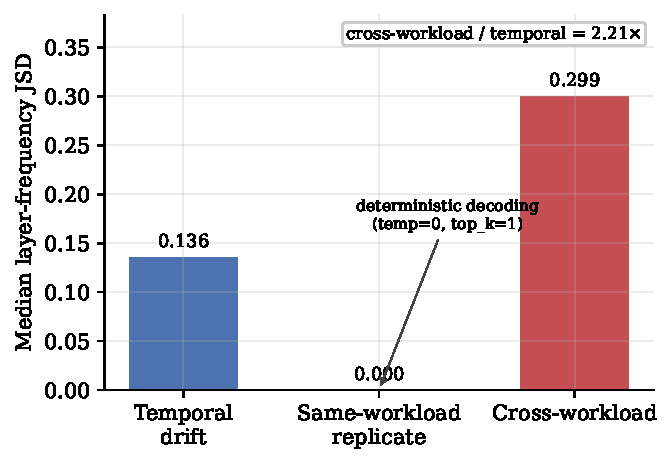
\includegraphics[width=0.68\linewidth]{figures/figure_b4_r2_08_scale_comparison.pdf}
\caption{R-08 scale comparison of median layer-frequency Jensen--Shannon
divergence (JSD): temporal drift within captures, same-workload replicate
divergence, and cross-workload divergence. The same-workload replicate bar
is $0.000$ under the deterministic decoding protocol (temperature~$=0.0$,
top-$k=1$) at the reported resolution; it is a reproducibility check, not
a general claim of zero stochastic variability.}
\label{fig:b4-scale}
\end{figure}

Table~\ref{tab:r2-08-summary} and Figure~\ref{fig:b4-scale} show that
cross-workload divergence dominates the predeclared comparison. Median
cross-workload JSD is $0.299$, median temporal JSD is $0.136$, and the
cross-workload/temporal ratio is $2.21\times$ (predeclared dominance
threshold $1.5\times$). The strongest tested workload pair is
\texttt{reasoning-v1} seed~42 versus \texttt{instruction-v1} seed~42
(median layer frequency JSD $0.421$). The predeclared regime is
\texttt{WORKLOAD\_DEPENDENCE\_DOMINANT}.

Under the deterministic decoding protocol, median same-workload replicate
JSD is $0.0$ at the reported resolution. This must be interpreted
narrowly: \emph{under the deterministic decoding protocol used here,
same-workload replicate frequency distributions were identical at the
reported resolution}. It is a reproducibility check, not evidence that
run-to-run stochastic variability is zero in general. The result
strengthens attribution of the observed differences to temporal position
and workload category within this protocol; it does not generalize beyond
this protocol.

\subsection{Synthesis and Connection to Causal Prediction}
\label{sec:iib-synthesis}

This evidence forms a constrained chain. R-05 shows that routing is
non-uniform, while canonical auxiliary R-03 evidence shows that static
LFU does not outperform Global-LRU at any tested capacity-constrained
point on the DEV trace (tying only at 16~GiB effective residency). R-06
shows that previous routing state carries measurable information about
subsequent routing. R-07 shows that this structure is
strongest at short horizons, with reuse and working sets more compact than
a shuffled null. R-08 shows that the routing signature varies materially
by workload under the tested protocol.

The central restrained claim is therefore:

\begin{quote}
\emph{Under the tested Qwen3-30B-A3B-Q4\_K\_M workload and runtime
protocol, expert routing exhibits substantial aggregate concentration,
measurable transition dependence, strong short-horizon reuse locality, and
pronounced workload dependence. These properties establish empirical
structure that can motivate causal working-set prediction, but do not
themselves demonstrate predictive accuracy or runtime improvement.}
\end{quote}

This characterization connects to the earlier analysis through the measured
clairvoyant-comparator gap, which measures the separation between a simple
causal baseline and the implemented comparator $O_B$; here we assess whether
observable routing history contains structure that could, in principle,
allow a stronger causal policy to reduce part of that measured gap.
The causal-prediction and real-runtime validation stage defines the signed
comparator-relative recovery metric
\begin{equation}
\label{eq:comparator-relative-recovery}
\mathrm{RecoveryOfBeladyGap}
  = \frac{B - P}{B - O_B},
\end{equation}
where $B$ is selected causal baseline miss bytes, $P$ is predictor-driven
miss bytes, and $O_B$ is implemented comparator miss bytes, all at fixed
budget and workload. The metric is signed; values $>1$ are possible under
CASE~C and mean $P$ beats $O_B$, not $O^*$. This metric is not populated
by the routing characterization, and the actual reported evaluation
(Section~\ref{sec:iic}) instead reports its predictor's performance via the
R-09B/R-10 held-out recall$@k$ margin and its retention policy's
performance via the frozen R-11/R-12 metrics
(miss bytes per decode step and decode tokens per second respectively),
which are the
metrics the frozen decision rules for that stage actually define and
apply; this equation is retained here as the originally-planned
connective metric between the earlier analyses and the causal-prediction
stage, not as a value that was ultimately computed and reported.